\section{Модификация проекта «Выпуклая оболочка»}

\subsection{Постановка задачи}
Требуется модифицировать эталонный проект:
\begin{itemize}
\item для индуктивного вычисления количества всех острых внутренних углов выпуклой
оболочки~(задача 40);
\item для индуктивного вычисления расстояния от выпуклой оболочки до заданного
стандартного прямоугольника~(Задача 52).
\end{itemize}

\subsection{Теоретические аспекты}

Задача построения выпуклой оболочки множества точек может быть сформулирована следующим
образом: для множества точек $M$ необходимо найти наименьшее \emph{выпуклое} множество,
включающее $M$. \emph{Выпуклым} будем называть любое множество $M$, удовлетворяющее условию:
$ \forall x_1, x_2 \in M\ [x_1,x_2]\in M.$

\begin{figure}[ht!]
\begin{center}
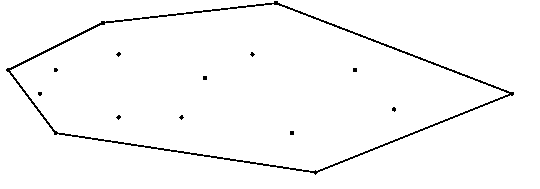
\includegraphics[scale=0.6]{images/conv_a_1}
\end{center}
\vspace*{-8mm}
\caption{Выпуклая оболочка множества точек}\label{fig:convex_hull}
\end{figure}

Пусть $X$~---множество точек на плоскости $\mathbb{R}^2$, $\mathcal{P}$~---
множество всех выпуклых фигур на плоскости. Тогда тройка $\left(f,g,h\right)$, где
$f\colon X^* \rightarrow \mathcal{P}$~---
\emph{выпуклая оболочка последовательности точек},
$g\colon X^* \rightarrow \mathbb{N}$~--- \emph{количество острых углов в ней},
$h\colon X^* \rightarrow \mathbb{R}$~---
\emph{расстояние от неё до стандартного прямоугольника}, задаёт индуктивную
функцию $$F\colon X^* \rightarrow \mathcal{P} \times \mathbb{N} \times
\mathbb{R},~F = \begin{pmatrix}f\\ g\\ h\end{pmatrix}\,.$$
Функция индуктивного перевычисления $G$ представляет собой реализацию следующей
идеи: пусть для некоторой последовательности точек $X^*$ значения $f,g,h$ уже известны.
Тогда при поступлении новой точки $x$ возможны два случая:
либо точка лежит внутри выпуклой оболочки, либо снаружи неё. Если $x$ внутри,
то её можно игнорировать, так как она не изменит характеристик выпуклой оболочки.
Рассмотрим случай, когда она находится снаружи. Для того, чтобы понять, удалять ребро или нет, воспользуемся критерием \emph{освещённости} ребра оболочки из этой точки~\ref{fig:conv_light}\,.
\begin{figure}[ht!]
\begin{center}
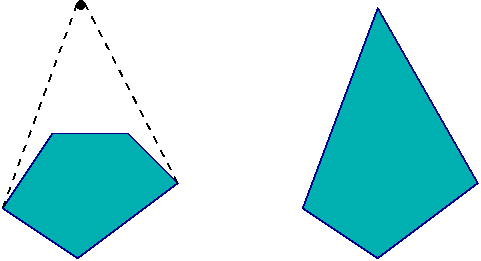
\includegraphics[scale=0.6]{images/conv_a_2}
\end{center}
\vspace*{-8mm}
\caption{Изменение выпуклой оболочки при добавлении точки}\label{fig:conv_light}
\end{figure}

Для получения новой оболочки необходимо удалить все освещённые рёбра, а концы
оставшейся ломаной соединить двумя новыми рёбрами с добавляемой точкой $x$.
Если добавляемая точка лежит на продолжении одного из рёбер, то оболочка должна
измениться, поэтому ребро, на продолжении которого лежит точка $x$, мы также будем
считать освещённым.

\newpage

Для вычисления функции $g$, количества острых углов в выпуклой оболочке, нам необходимо хранить \emph{множество} точек, углы при которых острые~(\verb|Set::@@angles| будем обозначать $A$). Случаи точки и двуугольника тривиальны (0 и 2 острых угла соответственно). Для треугольника достаточно напрямую проверить, являются ли углы острыми при помощи сравнения скалярного произведения с нулём (метод точки \verb|ac_angle?(a,b)|~--- двухместный предикат <<угол образуемый точкой~--- вершиной и точками \verb|a|, \verb|b|~--- острый>>) и если углы острые, добавить точки в множество $A$.

Для выпуклой оболочки из более чем 3 точек алгоритм вычисления количества острых углов такой: 
\begin{itemize}
\item если точка удаляется при добавлении новой вершины в выпуклую оболочку, удалить её из множества $A$;
\item после удаления всех освещённых из добавляемой вершины рёбер, следует добавить в $A$ вершины, смежные с добавленной и обладающие острым углом, и добавляемую вершину, если угол при ней острый. Естественно, также нужно исключить из $A$ те из смежных с новой вершиной точки, углы при которых не острые~(см.~рис.~\ref{fig:conv_light}).
\end{itemize}

Далее рассмотрим задачу вычисления функции $h$ расстояния от выпуклой оболочки до стандартного прямоугольника\footnote{Подробный код методов, решающих эту задачу, доступен в приложении.}\,.

Расчёт расстояния от точки до прямоугольника и от отрезка до прямоугольника как подзадача входит в задачу для выпуклой оболочки, поэтому здесь рассмотрен не будет. Рассмотрение метода вычисления расстояния до отрезка описано в разделе \emph{Используемые алгоритмы и структуры данных}. 

В случае треугольника достаточно вычислить расстояние от каждой стороны, если центр прямоугольника
 не лежит внутри треугольника; если центр внутри, то $g$ автоматически становится $0$, так как 
 выпуклая оболочка включает в себя свою внутренность.

Рассмотрим случай общей выпуклой оболочки:
учитывая, что расстояние до выпуклой оболочки может только уменьшаться, нам нужно лишь проверить, не попадает ли прямоугольник в получаемую при добавлении вершины область и вычислить расстояние до добавляемых отрезков.

Таким образом, мы знаем, как индуктивно вычислять расстояние от выпуклой оболочки до стандартного прямоугольника.

\begin{figure}[ht!]
\begin{center}
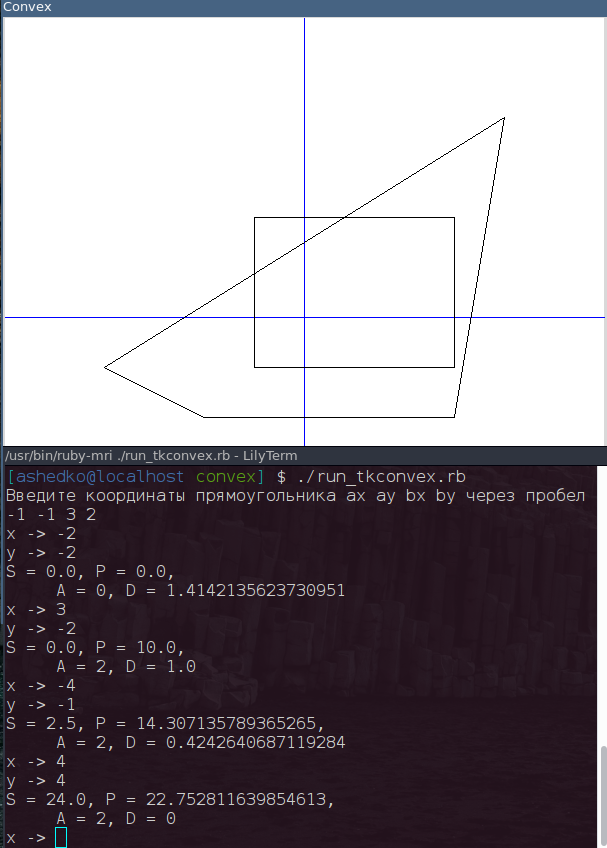
\includegraphics[scale=0.6]{images/convex_ill}
\end{center}
\vspace*{-8mm}
\caption{Иллюстрация работы программы}\label{fig:conv_ill}
\end{figure}

\newpage

\subsection{Используемые алгоритмы и структуры данных}

\textbf{Структуры данных}

При вычислении количества острых углов используется структура данных \emph{множество}. По своей сути она представляет собой хэш, в котором ключи и есть данные. В работе она используется из-за простоты добавления и удаления элементов, так как \verb|Set| в языке Ruby позволяет выполнять над собой стандартные теоретико-множественные операции.

\textbf{Вычисление расстояния от отрезка до прямоугольника}

Прежде, чем начать работу с отрезком, проверим его на пересечение с прямоугольником~(алгоритм описан ниже).
В начале вычислим положение концов отрезка относительно прямоугольника, воспользовавшись таблицей:
\begin{center}
\begin{tabular}{|c|c|}
\hline
Характеристика & Номер четверти \\
\hline 
$(\mathbf{0},\mathbf{0})$ & 0 \\ 
\hline 
$(\mathbf{0},\mathbf{1})$ & 1 \\
\hline
$(\mathbf{1},\mathbf{0})$ & 2 \\
\hline
$(\mathbf{1},\mathbf{1})$ & 3 \\
\hline
\end{tabular} 
\end{center}
где характеристика~--- результат сравнения координат точки с  координатами центра прямоугольника~(первая координата~--- горизонтальная, вторая~--- вертикальная\, (см.~рис. \ref{fig:conv_rect})).
\begin{figure}[ht!]
\begin{center}
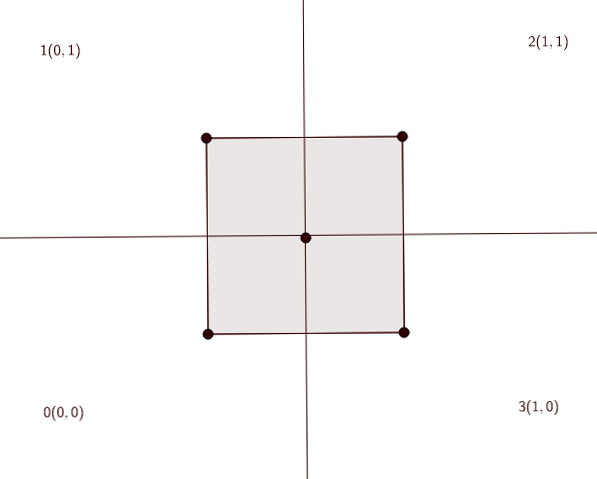
\includegraphics[scale=0.4]{images/conv_rect}
\end{center}
\vspace*{-8mm}
\caption{Разделение пространства вокруг прямоугольника}\label{fig:conv_rect}
\end{figure}

Затем проверим, не является ли отрезок точкой, и, если является, остаётся только проверить расстояние до ближайших двух сторон прямоугольника при помощи метода вычисления расстояния от точки до отрезка.

Если же отрезок невырожденный, возможно три случая его положения относительно прямоугольника~(рис. \ref{fig:conv_case}\,):
\begin{list}{a}{}
\item[\textbf{a})] оба конца лежат в одной четверти;
\item[\textbf{b})] концы в соседних четвертях;
\item[\textbf{c})] концы в противоположных четвертях.
\end{list}
В случае \textbf{a} необходимо вычислить расстояние от отрезка до ближайшей вершины прямоугольника и расстояния от концов отрезка до соответствующих им сторон прямоугольника\,(см.~приложение), после чего взять минимальное из них.
В случае \textbf{b} необходимо вычислить расстояние от отрезка до вершин прямоугольника в соответствующих четвертях и расстояния от концов отрезка до стороны прямоугольника. Далее, аналогично \textbf{a} взять минимум из них.
В случае \textbf{c} нужно всего лишь взять меньшее из расстояний от вершин, не лежащих в одной четверти с концами отрезка, до отрезка.
\begin{figure}[ht!]
\begin{center}
\textbf{a})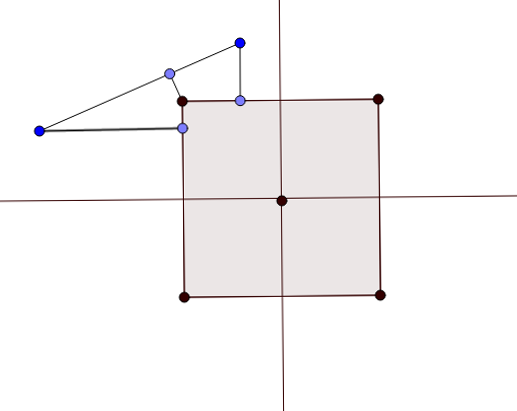
\includegraphics[scale=0.3]{images/conv_case1}
\vspace*{+10mm}
\textbf{b})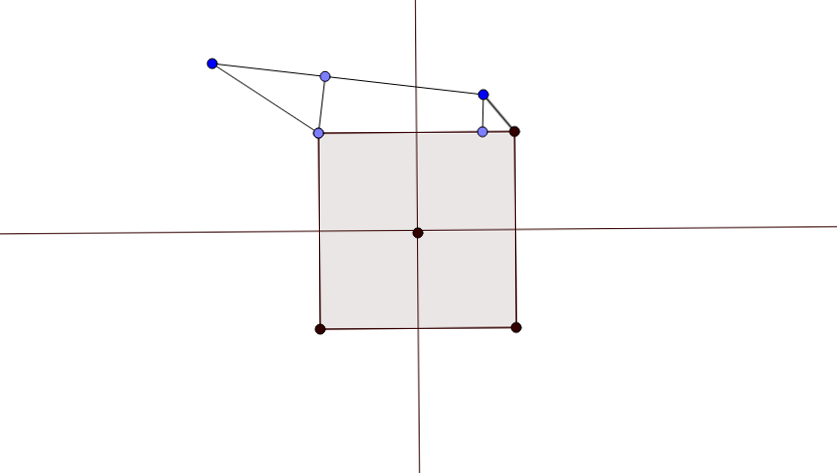
\includegraphics[scale=0.27]{images/conv_case2}
\textbf{c})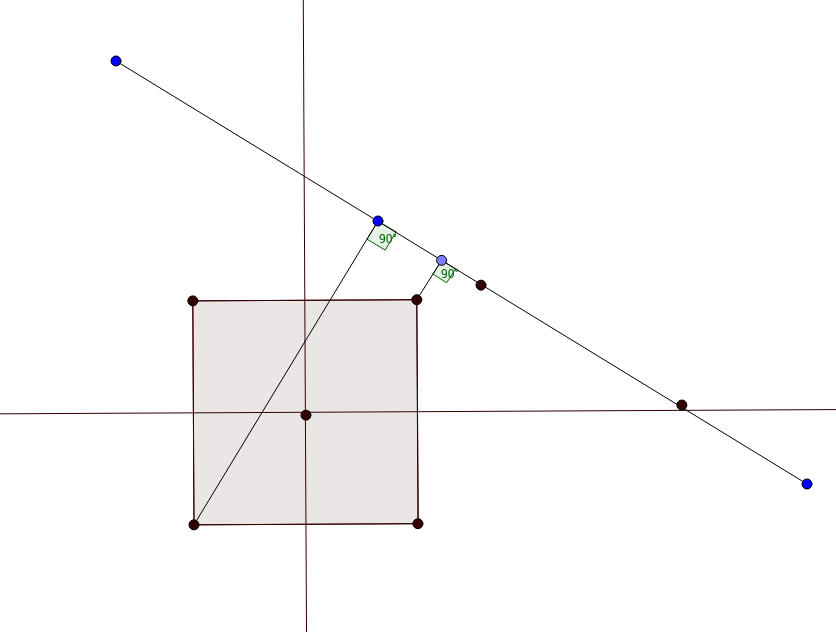
\includegraphics[scale=0.26]{images/conv_case3}
\end{center}
\vspace*{-8mm}
\caption{Различные варианты расположения точек}\label{fig:conv_case}
\end{figure}

Таким образом можно быстро находить расстояние от отрезка до прямоугольника. В данном случае задача упрощается тем, что, если отрезок целиком внутри прямоугольника, то расстояние до него равно $0$. 

По сравнению с <<лобовым>> методом вычисления приведённый выше алгоритм работает примерно в 3 раза быстрее (в <<лобовом>> методе производится $12$ операций вычисления длины, этот алгоритм позволяет ограничиться $4$).
Идея алгоритма автором найдена в заметках конференции, посвящённой базам данных \cite{seginters}\,.


\textbf{Вычисление пересечения отрезка и прямоугольника~(\emph{segment clipping})}

Алгоритм Лианга-Барского~\cite{barsky} использует параметрическое уравнение прямой и неравенства, описывающие прямоугольник~(clipping window), для вычисления пересечений между прямой и прямоугольником. С помощью этих пересечений можно выяснить, какая часть отрезка пересекает прямоугольник.

Параметрическое уравнение прямой:
$$
\begin{cases}
x = x_0 + u (x_1 - x_0) = x_0 + t \Delta x~,\\
y = y_0 + u (y_1 - y_0) = y_0 + t \Delta y~.\\
\end{cases}
$$

Точка находится внутри прямоугольника, если:
$$x_{\text{min}} \leqslant x_0 + t \Delta x \leqslant x_{\text{max}}~;$$
$$y_{\text{min}} \leqslant y_0 + t \Delta y \leqslant y_{\text{max}}\,\!.$$

Введём следующие обозначения:

\begin{tabular}{l}
$p_1 = -\Delta x  , q_1 = x_0 - x_{\text{min}}\,\!$~; \\
$p_2 = \Delta x  ,  q_2 = x_{\text{max}} - x_0\,\!$~;\\
$p_3 = -\Delta y , q_3 = y_0 - y_\text{min}\,\!$~;\\
$p_4 = \Delta y ,  q_4 = y_\text{max} - y_0\,\!~. $
\end{tabular}

\noindent Для получения пересечения, заметим следующее:
\begin{enumerate}
\item если отрезок параллелен $i$-тому ребру, $p_i=0$  для этого ребра;
\item если для этого $i,q_i<0$, отрезок полностью находится вне прямоугольника;
\item если $p_i<0$, отрезок направлен внутрь через это ребро, а если $p_i>0$~---наружу;
\item для $p_k\neq0$, $u={q_i}/{p_i}$ даёт точку пересечения.
\end{enumerate}
Метод вычисления $u_1$ и $u_2$: для $u_1$ рассмотреть рёбра, где  $p_i<0$, $u_1$~---  максимум из $\{0,q_i/p_i\}$; для $u_2$ рассмотреть 
рёбра, где $p_i>0$, $u_2$~--- минимум из $\left\{1,{q_i}/{p_i}\right\}$.
Если $u_1>u_2$, то отрезок находится снаружи и потому также не пересекает прямоугольник.


\subsection{Возможные обобщения}
В качестве более общей задачи можно рассматривать:
\begin{itemize}
\item задачу в пространстве произвольной размерности;
\item прямоугольник общего положения~(решается при помощи преобразования поворота и сдвига для координат точек);
\item поиск расстояния до других фигур~(круг, треугольник, произвольная область, ограниченная конечным числом ломаных).
\end{itemize}
